% Generated by tools/build_appendix.py from the analysis outputs. Do not edit by hand.
% Requires \\usepackage{booktabs,adjustbox,placeins} in the preamble.
\FloatBarrier
\section{Methods details}\label{app:methods}
\subsection{Windows, specifications and correction families}
All windows are half-open. The before period is November 1, 2024--April 14, 2025 and the after period is April 29--July 31, 2025; the corpus holds no data for April 28--30. The post-rollback slope is estimated over May 1--July 31, when every turn carries the label gpt-4.1-mini-2025-04-14. The event-window check compares April 15--23 with April 25--27. The 324-specification grid for each draw crosses four before windows (November 1--April 14; January 21--April 14; March 4--April 14; March 1--April 14), three after windows (April 29, May 13 or June 1 to July 31), three units (turn; mean per conversation $\times$ IP; first turn per conversation $\times$ IP), three length adjustments (none; log reply words; log user and reply words) and three template thresholds (below 100, 20 or 5 conversations sharing the opening). Standard errors are clustered on hashed IP throughout. Benjamini--Hochberg adjustment is applied across the 324 specifications within each draw, and within each set of seven criteria (each column of Table~2 and each traffic arm of the event-window contrasts). Weekly bins run Tuesday to Monday and are labelled by their end date; the final bin holds July 29--31. Changepoints use PELT with an $\ell_2$ cost, a minimum segment of two bins and penalty $\log(n)\,\mathrm{var}(\Delta y)/2$; support is the share of 500 parametric resamples of the weekly means in which a break recurs within 14 days.

\subsection{Templated traffic and the pool it is counted in}
A conversation is templated when at least 100 conversations share the first 500 characters of its opening user message (Section~3.2). Counts are taken over the WildChat-4.8M-Full conversations from November 1, 2024 onward (2,808,223 conversations), in which 631 openings reach the threshold and cover 44.4\% of conversations. Draws A and B exclude every conversation at or above the threshold before sampling. In the supporting sample, the pool count flags 46.6\% of conversations and 40.2\% of turns; counting within the 37,997-conversation sample instead would flag 33.7\% and 22.9\%, because applications that are thin in the sample still reach the threshold in the pool.

\subsection{Judges and prompts}
Draws A and B are scored for validation by Gemma 3 27B; the supporting sample is scored by Gemma 3 12B on six criteria and a holistic rating. Five criteria exist in two slightly different prompt wordings (``the AI chatbot'' and ``the AI assistant''); every comparison in the paper stays within one wording. The two judges are not on a common scale, so the paper compares only the direction and relative size of changes across them (Appendix~\ref{app:judges}).

\FloatBarrier
\section{Ordinary-traffic draws}\label{app:draws}
\begin{table}[h]
\caption{Samples. IPs are distinct hashed sender IPs.}
\label{tab:app-samples}
\footnotesize
\setlength{\tabcolsep}{4pt}
\begin{adjustbox}{max width=\linewidth}
\begin{tabular}{@{}lrrrrlr@{}}
\toprule
Sample & Turns drawn & Turns scored & Conversations & IPs & Span & Weeks \\
\midrule
Supporting sample (12B) & 65,292 & 65,292 & 37,997 & 26,364 & 2024-11-01 -- 2025-07-31 & 37 \\
Trend sample (12B) & 16,878 & 16,878 & 9,837 & 7,854 & 2023-04-09 -- 2025-07-31 & 119 \\
Ordinary Draw A (27B) & 80,468 & 80,143 & 36,397 & 23,218 & 2024-11-01 -- 2025-07-31 & 37 \\
Ordinary Draw B (27B) & 79,474 & 79,402 & 36,825 & 23,214 & 2024-11-01 -- 2025-07-31 & 37 \\
\bottomrule
\end{tabular}
\end{adjustbox}
\end{table}

\begin{table}[h]
\caption{Contrasts in validation points (27B), with 95\% intervals clustered on hashed IP. Era: before vs.\ after period. Length-adjusted rows report the adjusted difference; $d$ is given only for unadjusted contrasts.}
\label{tab:app-contrasts}
\footnotesize
\setlength{\tabcolsep}{4pt}
\begin{adjustbox}{max width=\linewidth}
\begin{tabular}{@{}llrrrrr@{}}
\toprule
Draw & Contrast & Turns & Means & Difference & $p$ & $d$ \\
\midrule
A & era, raw & 41,792 / 34,246 & 2.76 $\to$ 3.75 & +0.99 [0.76, 1.22] & $<$.001 & 0.40 \\
A & era, log assistant words & 41,792 / 34,246 & 2.76 $\to$ 3.75 & +0.86 [0.73, 1.00] & $<$.001 & -- \\
A & era, log user+assistant words & 41,792 / 34,246 & 2.76 $\to$ 3.75 & +0.95 [0.81, 1.09] & $<$.001 & -- \\
A & era, Mar 1-Apr 14 baseline & 16,399 / 34,246 & 2.79 $\to$ 3.75 & +0.96 [0.61, 1.31] & $<$.001 & 0.38 \\
A & era, empty openers dropped & 41,414 / 34,039 & 2.75 $\to$ 3.75 & +1.01 [0.78, 1.23] & $<$.001 & 0.40 \\
A & event window (Apr25-27 vs Apr15-23) & 3,153 / 737 & 3.69 $\to$ 3.96 & +0.26 [$-0.24$, 0.76] & .303 & 0.10 \\
A & transition (Apr15-23 vs Apr8-14) & 2,470 / 3,153 & 2.51 $\to$ 3.69 & +1.18 [0.89, 1.47] & $<$.001 & 0.50 \\
B & era, raw & 42,782 / 32,303 & 2.72 $\to$ 3.73 & +1.01 [0.80, 1.22] & $<$.001 & 0.41 \\
B & era, log assistant words & 42,782 / 32,303 & 2.72 $\to$ 3.73 & +0.89 [0.76, 1.02] & $<$.001 & -- \\
B & era, log user+assistant words & 42,782 / 32,303 & 2.72 $\to$ 3.73 & +0.99 [0.86, 1.12] & $<$.001 & -- \\
B & era, Mar 1-Apr 14 baseline & 16,362 / 32,303 & 2.72 $\to$ 3.73 & +1.01 [0.67, 1.35] & $<$.001 & 0.40 \\
B & era, empty openers dropped & 42,555 / 32,029 & 2.72 $\to$ 3.73 & +1.01 [0.80, 1.22] & $<$.001 & 0.41 \\
B & event window (Apr25-27 vs Apr15-23) & 3,265 / 753 & 3.76 $\to$ 3.44 & $-0.32$ [$-0.68$, 0.04] & .084 & $-0.13$ \\
B & transition (Apr15-23 vs Apr8-14) & 2,874 / 3,265 & 2.91 $\to$ 3.76 & +0.85 [0.49, 1.21] & $<$.001 & 0.34 \\
\bottomrule
\end{tabular}
\end{adjustbox}
\end{table}

\paragraph{Agreement between draws.} Across 37 weeks, the weekly means of Draws A and B correlate at $r = 0.945$ (Spearman $\rho = 0.880$) and differ by 0.15 points on average.

\begin{table}[h]
\caption{Post-rollback slope of validation per calendar week, May 1--July 31. Turn-level rows cluster on hashed IP; ``mix held fixed'' reweights each week to the before-period language $\times$ reply-length composition; weekly-means rows use the 12 non-empty weekly bins ending May 5--July 28 (the bin ending June 2 is empty; the corpus has no data May 26--June 6).}
\label{tab:app-slopes}
\footnotesize
\setlength{\tabcolsep}{4pt}
\begin{adjustbox}{max width=\linewidth}
\begin{tabular}{@{}llrrr@{}}
\toprule
Draw & Specification & $n$ & Slope [95\% CI] & $p$ \\
\midrule
A & Turns: raw & 34,246 & +0.059 [0.031, 0.087] & $<$.001 \\
A & Turns: + log assistant words & 34,246 & +0.042 [0.017, 0.067] & $<$.001 \\
A & Turns: + log assistant words + language & 34,246 & +0.050 [0.025, 0.075] & $<$.001 \\
A & Turns: + log user \& assistant words + language + turn index & 34,246 & +0.063 [0.035, 0.090] & $<$.001 \\
A & Turns: English only & 18,291 & +0.022 [$-0.014$, 0.058] & .230 \\
A & Turns: Non-English & 15,955 & +0.082 [0.046, 0.117] & $<$.001 \\
A & Turns: Reply length tercile: short & 9,012 & +0.012 [$-0.060$, 0.083] & .745 \\
A & Turns: Reply length tercile: medium & 12,752 & +0.068 [0.040, 0.095] & $<$.001 \\
A & Turns: Reply length tercile: long & 12,482 & +0.051 [0.018, 0.085] & .002 \\
A & Turns: lang x length tercile, pre-period weights & 34,246 & +0.032 [0.007, 0.056] & .013 \\
A & Weekly means, all turns, Newey--West 2 lags & 12 wk & +0.075 [0.036, 0.113] & $<$.001 \\
A & Weekly means, all turns, Newey--West 4 lags & 12 wk & +0.075 [0.041, 0.109] & $<$.001 \\
A & Weekly means, English turns, Newey--West 2 lags & 12 wk & +0.032 [0.010, 0.055] & .005 \\
A & Weekly means, English turns, Newey--West 4 lags & 12 wk & +0.032 [0.011, 0.053] & .002 \\
\midrule
B & Turns: raw & 32,303 & +0.055 [0.024, 0.086] & $<$.001 \\
B & Turns: + log assistant words & 32,303 & +0.039 [0.012, 0.067] & .005 \\
B & Turns: + log assistant words + language & 32,303 & +0.046 [0.019, 0.073] & $<$.001 \\
B & Turns: + log user \& assistant words + language + turn index & 32,303 & +0.060 [0.032, 0.088] & $<$.001 \\
B & Turns: English only & 15,447 & +0.037 [$-0.009$, 0.083] & .116 \\
B & Turns: Non-English & 16,856 & +0.060 [0.024, 0.096] & $<$.001 \\
B & Turns: Reply length tercile: short & 8,297 & +0.027 [$-0.040$, 0.094] & .425 \\
B & Turns: Reply length tercile: medium & 11,864 & +0.060 [0.028, 0.091] & $<$.001 \\
B & Turns: Reply length tercile: long & 12,142 & +0.043 [0.004, 0.081] & .032 \\
B & Turns: lang x length tercile, pre-period weights & 32,303 & +0.022 [$-0.006$, 0.050] & .122 \\
B & Weekly means, all turns, Newey--West 2 lags & 12 wk & +0.065 [0.042, 0.088] & $<$.001 \\
B & Weekly means, all turns, Newey--West 4 lags & 12 wk & +0.065 [0.043, 0.088] & $<$.001 \\
B & Weekly means, English turns, Newey--West 2 lags & 12 wk & +0.034 [0.008, 0.061] & .011 \\
B & Weekly means, English turns, Newey--West 4 lags & 12 wk & +0.034 [0.013, 0.055] & .001 \\
\bottomrule
\end{tabular}
\end{adjustbox}
\end{table}

\begin{table}[h]
\caption{Before--after change in validation within language and reply-length strata, and with the language $\times$ reply-length mix held at the before-period composition. Reply-length terciles are fixed on the before period.}
\label{tab:app-strata}
\footnotesize
\setlength{\tabcolsep}{4pt}
\begin{adjustbox}{max width=\linewidth}
\begin{tabular}{@{}llrrr@{}}
\toprule
Draw & Stratum & Turns & Change [95\% CI] & $p$ \\
\midrule
A & all & 76,038 & +0.99 [0.76, 1.22] & $<$.001 \\
A & English only & 38,015 & +1.00 [0.50, 1.50] & $<$.001 \\
A & Non-English & 38,023 & +0.95 [0.80, 1.10] & $<$.001 \\
A & Reply length tercile: short & 23,042 & +1.13 [0.66, 1.59] & $<$.001 \\
A & Reply length tercile: medium & 26,584 & +0.73 [0.56, 0.90] & $<$.001 \\
A & Reply length tercile: long & 26,412 & +1.00 [0.81, 1.20] & $<$.001 \\
A & lang x length tercile, pre-period weights & 76,038 & +0.82 [0.63, 1.02] & $<$.001 \\
B & all & 75,085 & +1.01 [0.80, 1.22] & $<$.001 \\
B & English only & 35,022 & +1.09 [0.66, 1.51] & $<$.001 \\
B & Non-English & 40,063 & +0.94 [0.78, 1.09] & $<$.001 \\
B & Reply length tercile: short & 22,599 & +1.20 [0.79, 1.61] & $<$.001 \\
B & Reply length tercile: medium & 26,101 & +0.78 [0.61, 0.95] & $<$.001 \\
B & Reply length tercile: long & 26,385 & +0.97 [0.78, 1.17] & $<$.001 \\
B & lang x length tercile, pre-period weights & 75,085 & +0.87 [0.68, 1.06] & $<$.001 \\
\bottomrule
\end{tabular}
\end{adjustbox}
\end{table}

\begin{table}[h]
\caption{Returning users: IPs seen both before April 15 and after the rollback, each compared only with itself.}
\label{tab:app-within}
\footnotesize
\setlength{\tabcolsep}{4pt}
\begin{adjustbox}{max width=\linewidth}
\begin{tabular}{@{}llrrr@{}}
\toprule
Draw & Specification & IPs & Change [95\% CI] & $p$ \\
\midrule
A & fixed effect, turns & 167 & +1.11 [0.49, 1.73] & $<$.001 \\
A & fixed effect, + log reply length + language + turn index & 167 & +0.76 [0.41, 1.12] & $<$.001 \\
A & fixed effect, without five heaviest IPs & 162 & +0.36 [$-0.12$, 0.84] & .143 \\
A & fixed effect, English-language turns & 97 & +0.97 [0.35, 1.58] & .002 \\
A & each IP weighted equally (64\% of IPs higher) & 167 & +0.46 [0.14, 0.79] & .006 \\
B & fixed effect, turns & 194 & +1.07 [0.35, 1.79] & .004 \\
B & fixed effect, + log reply length + language + turn index & 194 & +0.62 [0.24, 0.99] & .001 \\
B & fixed effect, without five heaviest IPs & 189 & +0.11 [$-0.44$, 0.66] & .697 \\
B & fixed effect, English-language turns & 114 & +0.86 [0.12, 1.60] & .023 \\
B & each IP weighted equally (58\% of IPs higher) & 194 & +0.38 [0.02, 0.75] & .043 \\
\bottomrule
\end{tabular}
\end{adjustbox}
\par\smallskip\footnotesize Returning IPs: 167 of 13,650 (A) and 194 of 13,654 (B) before-period IPs; 19.9\% and 17.6\% of after-period turns; the five heaviest produce 50\% and 51\% of returning turns. Mean validation (A / B): leavers 2.80 / 2.75; returning before 2.55 / 2.54; returning after 4.02 / 3.96; joiners 3.68 / 3.68.
\end{table}

\begin{table}[h]
\caption{Composition of the draws after the rollback: first and last three complete weeks, and Spearman correlation with week.}
\label{tab:app-composition}
\footnotesize
\setlength{\tabcolsep}{4pt}
\begin{adjustbox}{max width=\linewidth}
\begin{tabular}{@{}llrrrr@{}}
\toprule
Draw & Measure & First 3 wk & Last 3 wk & $\rho$ & $p$ \\
\midrule
A & Validation (27B) & 3.08 & 3.90 & 0.66 & .020 \\
A & Turns per conversation & 1.64 & 3.99 & 0.92 & $<$.001 \\
A & English-language turns (\%) & 32.59 & 63.19 & 0.97 & $<$.001 \\
A & Median reply words & 112.50 & 200.67 & 0.54 & .073 \\
B & Validation (27B) & 3.16 & 3.87 & 0.73 & .007 \\
B & Turns per conversation & 1.53 & 3.77 & 0.94 & $<$.001 \\
B & English-language turns (\%) & 31.98 & 57.81 & 0.96 & $<$.001 \\
B & Median reply words & 109.83 & 198.00 & 0.66 & .018 \\
\bottomrule
\end{tabular}
\end{adjustbox}
\end{table}

\begin{table}[h]
\caption{Segments around the April dip.}
\label{tab:app-dip}
\footnotesize
\setlength{\tabcolsep}{4pt}
\begin{adjustbox}{max width=\linewidth}
\begin{tabular}{@{}llrrrrr@{}}
\toprule
Draw & Segment & Turns & Validation & English & Turns/conv. & Median reply words \\
\midrule
A & pre (Nov 1-Apr 14) & 41,792 & 2.76 & 47\% & 1.91 & 132 \\
A & Apr 15-27 & 4,105 & 3.74 & 52\% & 2.30 & 122 \\
A & Apr 29-May 19 & 5,155 & 3.10 & 33\% & 1.65 & 114 \\
A & May 20-Jul 31 & 29,091 & 3.87 & 57\% & 2.97 & 171 \\
B & pre (Nov 1-Apr 14) & 42,782 & 2.72 & 46\% & 1.93 & 131 \\
B & Apr 15-27 & 4,317 & 3.74 & 54\% & 2.38 & 121 \\
B & Apr 29-May 19 & 4,826 & 3.16 & 32\% & 1.52 & 106 \\
B & May 20-Jul 31 & 27,477 & 3.83 & 51\% & 2.81 & 181 \\
\bottomrule
\end{tabular}
\end{adjustbox}
\par\smallskip\footnotesize Draw A: Apr 15-27 vs.\ Apr 29-May 19 $-0.63$ [$-0.97$, $-0.29$]; Draw A: pre (Nov 1-Apr 14) vs.\ Apr 29-May 19 +0.34 [$-0.01$, 0.69]; Draw A: Apr 29-May 19 vs.\ May 20-Jul 31 +0.76 [0.47, 1.06]; Draw B: Apr 15-27 vs.\ Apr 29-May 19 $-0.58$ [$-0.89$, $-0.27$]; Draw B: pre (Nov 1-Apr 14) vs.\ Apr 29-May 19 +0.44 [0.12, 0.77]; Draw B: Apr 29-May 19 vs.\ May 20-Jul 31 +0.67 [0.38, 0.96]. Draw A: of 118 equally long window pairs placed before April 15, 8\% show a change at least as large in either direction and 0\% a drop at least as large; among English-language turns the dip is +0.07. Draw B: of 118 equally long window pairs placed before April 15, 12\% show a change at least as large in either direction and 0\% a drop at least as large; among English-language turns the dip is $-0.13$.
\end{table}

\begin{table}[h]
\caption{Changepoints in weekly mean validation (bin end date, bootstrap support).}
\label{tab:app-changepoints}
\footnotesize
\setlength{\tabcolsep}{4pt}
\begin{adjustbox}{max width=\linewidth}
\begin{tabular}{@{}llp{0.55\linewidth}@{}}
\toprule
Series & Weekly mean over & Breaks \\
\midrule
All traffic, supporting sample (12B) & turn & 2025-01-06 (100\%); 2025-02-24 (100\%); 2025-04-28 (100\%); 2025-06-09 (100\%); 2025-07-21 (100\%) \\
All traffic, supporting sample (12B) & cluster\_mean & 2025-01-06 (100\%); 2025-02-24 (100\%); 2025-04-28 (100\%); 2025-05-26 (100\%); 2025-07-21 (100\%) \\
Templated removed, supporting sample (12B) & turn & 2024-12-30 (99\%); 2025-02-03 (100\%); 2025-02-24 (100\%); 2025-04-21 (100\%); 2025-05-26 (73\%) \\
Templated removed, supporting sample (12B) & cluster\_mean & 2024-11-25 (82\%); 2024-12-30 (74\%); 2025-02-03 (100\%); 2025-02-24 (100\%); 2025-03-10 (100\%); 2025-03-31 (55\%); 2025-06-09 (80\%) \\
Ordinary Draw A (27B) & turn & 2024-11-18 (100\%); 2024-12-02 (100\%); 2025-04-21 (100\%); 2025-05-05 (100\%); 2025-05-26 (100\%) \\
Ordinary Draw A (27B) & cluster\_mean & 2024-11-18 (96\%); 2025-02-03 (100\%); 2025-03-10 (100\%); 2025-03-31 (100\%); 2025-05-26 (100\%) \\
Ordinary Draw B (27B) & turn & 2024-11-18 (100\%); 2024-12-09 (100\%); 2025-04-21 (100\%); 2025-05-05 (100\%); 2025-05-26 (100\%) \\
Ordinary Draw B (27B) & cluster\_mean & 2024-11-18 (100\%); 2025-02-03 (100\%); 2025-03-10 (100\%); 2025-03-31 (98\%); 2025-04-21 (95\%); 2025-05-05 (95\%); 2025-05-26 (81\%) \\
\bottomrule
\end{tabular}
\end{adjustbox}
\end{table}

\begin{table}[h]
\caption{Turns in the draws whose opening is shared by 20--99 or 5--99 conversations in the pool.}
\label{tab:app-near}
\footnotesize
\setlength{\tabcolsep}{4pt}
\begin{adjustbox}{max width=\linewidth}
\begin{tabular}{@{}lrrrr@{}}
\toprule
Draw & Period & Turns & 20--99 & 5--99 \\
\midrule
A & pre & 41,792 & 8.4\% & 16.2\% \\
A & post & 34,246 & 7.8\% & 17.6\% \\
A & all & 80,143 & 8.2\% & 16.6\% \\
B & pre & 42,782 & 7.6\% & 15.7\% \\
B & post & 32,303 & 7.4\% & 16.3\% \\
B & all & 79,402 & 7.5\% & 15.9\% \\
\bottomrule
\end{tabular}
\end{adjustbox}
\end{table}

\begin{figure}[h]
\centering
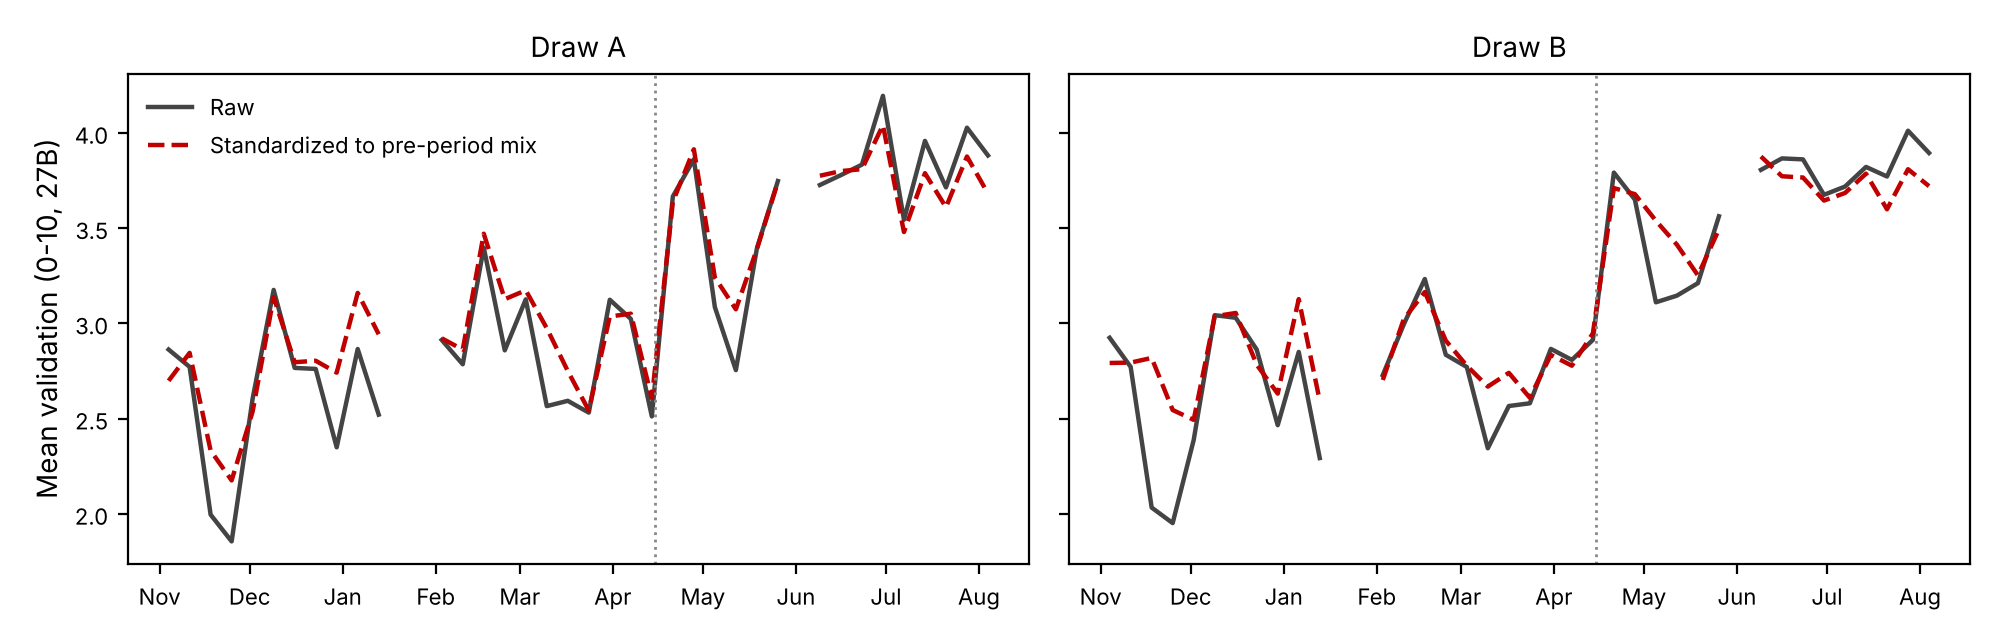
\includegraphics[width=\linewidth]{figures/appendix_raw_vs_standardized.png}
\caption{Weekly mean validation in each draw, raw and reweighted to the before-period language $\times$ reply-length composition. The dotted line marks April 15.}
\label{fig:app-standardized}
\end{figure}

\FloatBarrier
\section{Judges}\label{app:judges}
\begin{table}[h]
\caption{Validation scored by both judges on the same turns.}
\label{tab:app-judges}
\footnotesize
\setlength{\tabcolsep}{4pt}
\begin{adjustbox}{max width=\linewidth}
\begin{tabular}{@{}lrrrrrrrr@{}}
\toprule
Overlap & Turns & $r$ & $\rho$ & Identical & Within 1 & 12B & 27B & 27B$-$12B \\
\midrule
A & 3,298 & 0.68 & 0.72 & 44.4\% & 68.5\% & 3.87 & 2.78 & $-1.09$ \\
B & 3,324 & 0.68 & 0.71 & 40.3\% & 67.2\% & 4.11 & 3.07 & $-1.04$ \\
A or B (unique turns) & 6,293 & 0.68 & 0.71 & 40.2\% & 66.9\% & 4.12 & 3.06 & $-1.05$ \\
\bottomrule
\end{tabular}
\end{adjustbox}
\par\smallskip\footnotesize By reply-length tercile (Draw A overlap), 27B$-$12B: short $-0.88$ ($r = 0.63$); mid $-0.63$ ($r = 0.79$); long $-1.74$ ($r = 0.56$). Weekly series, supporting sample with templated traffic removed (12B) vs.\ each draw (27B): Draw A $r = 0.81$ over 37 weeks; Draw B $r = 0.84$ over 37 weeks.
\end{table}

\FloatBarrier
\section{Supporting sample: six criteria}\label{app:criteria}
\begin{table}[h]
\caption{Ordinary traffic in the supporting sample (12B), before vs.\ after, under four template rules. Intervals clustered on hashed IP. $^\dagger$ not significant after Benjamini--Hochberg adjustment within the column and rule.}
\label{tab:app-criteria}
\footnotesize
\setlength{\tabcolsep}{4pt}
\begin{adjustbox}{max width=\linewidth}
\begin{tabular}{@{}lrrrrr@{}}
\toprule
Criterion & Turns & Change [95\% CI] & $d$ & Length-adj. & Slope/week [95\% CI] \\
\midrule
\multicolumn{6}{@{}l}{\textit{Opening shared by fewer than 100 conversations (main)}} \\
Validation & 31,479 / 6,667 & +0.96 [0.64, 1.29] & 0.32 & +0.79 & +0.064 [$-0.002$, 0.129]$^\dagger$ \\
Agreement & 31,483 / 6,666 & +0.21 [0.01, 0.41] & 0.08 & +0.18$^\dagger$ & $-0.030$ [$-0.066$, 0.007]$^\dagger$ \\
Disagreement & 31,481 / 6,667 & +0.06 [$-0.10$, 0.22]$^\dagger$ & 0.03 & +0.01$^\dagger$ & +0.045 [0.012, 0.078]$^\dagger$ \\
Flattery & 31,481 / 6,668 & +0.59 [0.35, 0.83] & 0.31 & +0.45 & +0.039 [0.003, 0.075]$^\dagger$ \\
Enthusiasm & 31,478 / 6,669 & +0.75 [0.50, 1.00] & 0.29 & +0.60 & +0.044 [$-0.010$, 0.098]$^\dagger$ \\
Positive affirmation & 31,481 / 6,665 & +0.96 [0.65, 1.27] & 0.29 & +0.76 & +0.082 [0.014, 0.149]$^\dagger$ \\
Holistic (1--5) & 31,489 / 6,671 & $-0.08$ [$-0.21$, 0.04]$^\dagger$ & $-0.12$ & $-0.02$$^\dagger$ & $-0.006$ [$-0.015$, 0.004]$^\dagger$ \\
\multicolumn{6}{@{}l}{\textit{Fewer than 20}} \\
Validation & 29,023 / 6,276 & +0.99 [0.67, 1.31] & 0.33 & +0.81 & +0.059 [$-0.010$, 0.127]$^\dagger$ \\
Agreement & 29,025 / 6,276 & +0.24 [0.03, 0.45] & 0.09 & +0.20$^\dagger$ & $-0.037$ [$-0.075$, 0.002]$^\dagger$ \\
Disagreement & 29,024 / 6,276 & +0.03 [$-0.14$, 0.20]$^\dagger$ & 0.01 & $-0.03$$^\dagger$ & +0.054 [0.019, 0.089] \\
Flattery & 29,024 / 6,277 & +0.56 [0.32, 0.80] & 0.30 & +0.42 & +0.041 [0.004, 0.078]$^\dagger$ \\
Enthusiasm & 29,024 / 6,278 & +0.76 [0.51, 1.00] & 0.29 & +0.60 & +0.042 [$-0.013$, 0.098]$^\dagger$ \\
Positive affirmation & 29,026 / 6,275 & +0.99 [0.68, 1.30] & 0.30 & +0.78 & +0.079 [0.008, 0.151]$^\dagger$ \\
Holistic (1--5) & 29,029 / 6,279 & $-0.07$ [$-0.19$, 0.06]$^\dagger$ & $-0.10$ & $-0.01$$^\dagger$ & $-0.004$ [$-0.013$, 0.005]$^\dagger$ \\
\multicolumn{6}{@{}l}{\textit{Fewer than 5}} \\
Validation & 26,421 / 5,763 & +1.08 [0.79, 1.37] & 0.36 & +0.89 & +0.037 [$-0.022$, 0.095]$^\dagger$ \\
Agreement & 26,421 / 5,763 & +0.14 [$-0.07$, 0.34]$^\dagger$ & 0.05 & +0.11$^\dagger$ & $-0.032$ [$-0.072$, 0.007]$^\dagger$ \\
Disagreement & 26,421 / 5,763 & +0.12 [$-0.05$, 0.28]$^\dagger$ & 0.06 & +0.06$^\dagger$ & +0.053 [0.017, 0.088] \\
Flattery & 26,421 / 5,764 & +0.62 [0.39, 0.85] & 0.34 & +0.47 & +0.032 [$-0.002$, 0.065]$^\dagger$ \\
Enthusiasm & 26,422 / 5,765 & +0.79 [0.56, 1.02] & 0.31 & +0.62 & +0.031 [$-0.020$, 0.083]$^\dagger$ \\
Positive affirmation & 26,423 / 5,762 & +1.08 [0.77, 1.38] & 0.33 & +0.85 & +0.063 [$-0.006$, 0.132]$^\dagger$ \\
Holistic (1--5) & 26,424 / 5,765 & $-0.08$ [$-0.20$, 0.05]$^\dagger$ & $-0.11$ & $-0.01$$^\dagger$ & $-0.001$ [$-0.008$, 0.007]$^\dagger$ \\
\multicolumn{6}{@{}l}{\textit{Fewer than 100, bare greetings kept}} \\
Validation & 33,147 / 6,949 & +0.92 [0.60, 1.24] & 0.30 & +0.76 & +0.065 [0.001, 0.128]$^\dagger$ \\
Agreement & 33,151 / 6,948 & +0.21 [0.02, 0.40] & 0.08 & +0.19$^\dagger$ & $-0.028$ [$-0.064$, 0.007]$^\dagger$ \\
Disagreement & 33,148 / 6,949 & +0.05 [$-0.10$, 0.21]$^\dagger$ & 0.03 & +0.00$^\dagger$ & +0.044 [0.012, 0.076] \\
Flattery & 33,149 / 6,950 & +0.56 [0.33, 0.79] & 0.29 & +0.43 & +0.038 [0.003, 0.073]$^\dagger$ \\
Enthusiasm & 33,146 / 6,951 & +0.72 [0.48, 0.97] & 0.28 & +0.59 & +0.045 [$-0.008$, 0.098]$^\dagger$ \\
Positive affirmation & 33,148 / 6,947 & +0.92 [0.62, 1.22] & 0.28 & +0.73 & +0.083 [0.017, 0.149] \\
Holistic (1--5) & 33,157 / 6,953 & $-0.08$ [$-0.20$, 0.04]$^\dagger$ & $-0.11$ & $-0.02$$^\dagger$ & $-0.006$ [$-0.015$, 0.004]$^\dagger$ \\
\bottomrule
\end{tabular}
\end{adjustbox}
\end{table}

\begin{table}[h]
\caption{The 29 templates with at least 100 conversations in the supporting sample. Applications are not named; both extremes of mean validation are moderation classifiers that reply with a single word.}
\label{tab:app-templates}
\footnotesize
\setlength{\tabcolsep}{4pt}
\begin{adjustbox}{max width=\linewidth}
\begin{tabular}{@{}lrrr@{}}
\toprule
Rank & Turns & Conversations & Mean validation (12B) \\
\midrule
1 & 4,124 & 3,162 & 0.01 \\
2 & 3,271 & 2,692 & 0.22 \\
3 & 2,697 & 2,676 & 7.11 \\
4 & 680 & 587 & 9.47 \\
5 & 422 & 100 & 0.72 \\
6 & 266 & 249 & 9.29 \\
7 & 226 & 226 & 8.24 \\
8 & 215 & 215 & 4.67 \\
9 & 207 & 207 & 8.54 \\
10 & 202 & 197 & 4.68 \\
11 & 200 & 175 & 2.98 \\
12 & 189 & 179 & 0.28 \\
13 & 183 & 152 & 1.09 \\
14 & 162 & 101 & 6.09 \\
15 & 159 & 159 & 6.31 \\
16 & 147 & 147 & 4.54 \\
17 & 147 & 147 & 4.28 \\
18 & 143 & 119 & 9.62 \\
19 & 143 & 143 & 4.36 \\
20 & 134 & 133 & 6.66 \\
21 & 131 & 131 & 7.34 \\
22 & 131 & 131 & 4.23 \\
23 & 127 & 127 & 4.61 \\
24 & 124 & 124 & 3.40 \\
25 & 121 & 121 & 4.36 \\
26 & 110 & 110 & 7.99 \\
27 & 106 & 106 & 0.42 \\
28 & 102 & 102 & 6.30 \\
29 & 101 & 101 & 5.54 \\
\bottomrule
\end{tabular}
\end{adjustbox}
\end{table}

\FloatBarrier
\section{All traffic and the April event window}\label{app:alltraffic}
\begin{table}[h]
\caption{Event (April 25--27) and post-rollback (May 1--14) windows against April 15--23, all traffic (12B). Cohen's $d$ with 95\% intervals clustered on hashed IP; $p$ adjusted within each family of seven.}
\label{tab:app-event-all}
\footnotesize
\setlength{\tabcolsep}{4pt}
\begin{adjustbox}{max width=\linewidth}
\begin{tabular}{@{}lrrrrrrr@{}}
\toprule
Criterion & Base & Event & Post & Event $d$ & $p$ & Post $d$ & $p$ \\
\midrule
Validation & 4.14 & 6.20 & 4.21 & +0.57 [0.46, 0.68] & $<$.001 & +0.02 [$-0.09$, 0.13] & .691 \\
Agreement & 9.25 & 8.70 & 8.76 & $-0.28$ [$-0.42$, $-0.15$] & $<$.001 & $-0.26$ [$-0.37$, $-0.15$] & $<$.001 \\
Disagreement & 0.82 & 2.21 & 0.86 & +0.66 [0.53, 0.79] & $<$.001 & +0.02 [$-0.06$, 0.10] & .691 \\
Flattery & 1.47 & 3.11 & 1.73 & +0.68 [0.54, 0.83] & $<$.001 & +0.12 [0.01, 0.23] & .056 \\
Enthusiasm & 3.88 & 5.78 & 4.83 & +0.66 [0.53, 0.79] & $<$.001 & +0.36 [0.23, 0.49] & $<$.001 \\
Positive affirmation & 2.82 & 5.45 & 3.24 & +0.72 [0.59, 0.86] & $<$.001 & +0.12 [0.02, 0.23] & .050 \\
Holistic (1--5) & 3.84 & 3.44 & 3.86 & $-0.77$ [$-0.91$, $-0.63$] & $<$.001 & +0.02 [$-0.09$, 0.13] & .691 \\
\bottomrule
\end{tabular}
\end{adjustbox}
\end{table}

\begin{table}[h]
\caption{Event (April 25--27) and post-rollback (May 1--14) windows against April 15--23, templated conversations removed (12B). Cohen's $d$ with 95\% intervals clustered on hashed IP; $p$ adjusted within each family of seven.}
\label{tab:app-event-removed}
\footnotesize
\setlength{\tabcolsep}{4pt}
\begin{adjustbox}{max width=\linewidth}
\begin{tabular}{@{}lrrrrrrr@{}}
\toprule
Criterion & Base & Event & Post & Event $d$ & $p$ & Post $d$ & $p$ \\
\midrule
Validation & 4.82 & 4.34 & 4.14 & $-0.16$ [$-0.45$, 0.13] & .394 & $-0.22$ [$-0.45$, 0.01] & .122 \\
Agreement & 8.53 & 8.57 & 9.05 & +0.01 [$-0.34$, 0.36] & .979 & +0.21 [0.03, 0.39] & .122 \\
Disagreement & 1.02 & 1.03 & 0.78 & +0.00 [$-0.26$, 0.27] & .979 & $-0.12$ [$-0.28$, 0.04] & .162 \\
Flattery & 2.17 & 1.80 & 1.75 & $-0.17$ [$-0.49$, 0.14] & .394 & $-0.20$ [$-0.42$, 0.03] & .122 \\
Enthusiasm & 4.70 & 4.28 & 4.16 & $-0.16$ [$-0.45$, 0.12] & .394 & $-0.20$ [$-0.42$, 0.02] & .122 \\
Positive affirmation & 4.23 & 3.48 & 3.58 & $-0.23$ [$-0.53$, 0.08] & .394 & $-0.19$ [$-0.40$, 0.03] & .122 \\
Holistic (1--5) & 3.86 & 3.97 & 3.95 & +0.17 [$-0.13$, 0.47] & .394 & +0.14 [$-0.06$, 0.33] & .165 \\
\bottomrule
\end{tabular}
\end{adjustbox}
\end{table}

\begin{table}[h]
\caption{Event-window contrast after removing templated traffic, by pool threshold (12B).}
\label{tab:app-threshold}
\footnotesize
\setlength{\tabcolsep}{4pt}
\begin{adjustbox}{max width=\linewidth}
\begin{tabular}{@{}lrrrrr@{}}
\toprule
Removed if shared by & Templated, base / event & Turns left & Validation $d$ & Sig.\ increases & Sig.\ decreases \\
\midrule
$\geq$100 & 61.4\% / 86.2\% & 801 / 61 & $-0.16$ [$-0.45$, 0.13] & 0 & 0 \\
$\geq$50 & 62.9\% / 86.7\% & 770 / 59 & $-0.23$ [$-0.52$, 0.05] & 0 & 0 \\
$\geq$20 & 66.8\% / 88.5\% & 689 / 51 & $-0.35$ [$-0.66$, $-0.05$] & 0 & 0 \\
$\geq$10 & 68.1\% / 88.9\% & 663 / 49 & $-0.30$ [$-0.61$, 0.01] & 0 & 0 \\
$\geq$5 & 69.9\% / 89.4\% & 626 / 47 & $-0.32$ [$-0.64$, $-0.01$] & 0 & 0 \\
$\geq$3 & 70.6\% / 90.0\% & 610 / 44 & $-0.38$ [$-0.70$, $-0.06$] & 0 & 4 \\
\bottomrule
\end{tabular}
\end{adjustbox}
\end{table}

\begin{table}[h]
\caption{Templated traffic in the April windows and the largest application in each.}
\label{tab:app-clients}
\footnotesize
\setlength{\tabcolsep}{4pt}
\begin{adjustbox}{max width=\linewidth}
\begin{tabular}{@{}lrrrrr@{}}
\toprule
Window & Turns & Templated & Templates & Largest, \% of window & Its validation \\
\midrule
baseline Apr15-23 & 2,077 & 61.4\% & 38 & 17.7\% & 0.38 \\
event Apr25-27 & 442 & 86.2\% & 25 & 57.0\% & 7.19 \\
post May1-14 & 4,054 & 59.1\% & 55 & 24.2\% & 3.01 \\
\bottomrule
\end{tabular}
\end{adjustbox}
\end{table}

\begin{table}[h]
\caption{Concentration of turns among IPs before and after the rollback.}
\label{tab:app-concentration}
\footnotesize
\setlength{\tabcolsep}{4pt}
\begin{adjustbox}{max width=\linewidth}
\begin{tabular}{@{}llrrrr@{}}
\toprule
Frame & Period & Turns & IPs & Largest IP & Five largest \\
\midrule
supporting, all traffic & before & 42,897 & 16,998 & 6.7\% & 10.7\% \\
supporting, all traffic & after & 19,660 & 7,501 & 38.9\% & 41.3\% \\
supporting, ordinary ($<$100) & before & 31,508 & 10,336 & 8.2\% & 12.0\% \\
supporting, ordinary ($<$100) & after & 6,680 & 2,456 & 2.6\% & 8.2\% \\
Draw A & before & 41,792 & 13,650 & 7.7\% & 11.2\% \\
Draw A & after & 34,246 & 8,642 & 2.8\% & 9.2\% \\
Draw B & before & 42,782 & 13,654 & 7.4\% & 10.4\% \\
Draw B & after & 32,303 & 8,613 & 3.1\% & 9.6\% \\
\bottomrule
\end{tabular}
\end{adjustbox}
\end{table}

\begin{table}[h]
\caption{Weeks in which at least two of the six criteria break, all traffic (12B).}
\label{tab:app-cp-all}
\footnotesize
\setlength{\tabcolsep}{4pt}
\begin{adjustbox}{max width=\linewidth}
\begin{tabular}{@{}lrp{0.38\linewidth}l@{}}
\toprule
Dates observed & Criteria & Which & Support \\
\midrule
2024-11-12 to 2024-11-18 & 2 & Agree, Disagree & 100\%, 100\% \\
2024-11-26 to 2024-12-02 & 2 & Agree, Disagree & 100\%, 100\% \\
2024-12-31 to 2025-01-06 & 2 & Validation, Positive affirmation & 100\%, 94\% \\
2025-02-18 to 2025-02-24 & 2 & Validation, Positive affirmation & 100\%, 95\% \\
2025-04-22 to 2025-04-27 & 4 & Validation, Disagree, Flatter, Enthusiasm & 100\%, 62\%, 100\%, 100\% \\
2025-05-06 to 2025-05-12 & 3 & Agree, Flatter, Enthusiasm & 99\%, 100\%, 100\% \\
2025-07-15 to 2025-07-21 & 4 & Validation, Disagree, Enthusiasm, Positive affirmation & 100\%, 63\%, 100\%, 100\% \\
\bottomrule
\end{tabular}
\end{adjustbox}
\end{table}

\begin{table}[h]
\caption{Weeks in which at least two of the six criteria break, templated conversations removed (12B).}
\label{tab:app-cp-removed}
\footnotesize
\setlength{\tabcolsep}{4pt}
\begin{adjustbox}{max width=\linewidth}
\begin{tabular}{@{}lrp{0.38\linewidth}l@{}}
\toprule
Dates observed & Criteria & Which & Support \\
\midrule
2024-11-12 to 2024-11-18 & 2 & Agree, Disagree & 100\%, 100\% \\
2024-11-26 to 2024-12-02 & 2 & Agree, Disagree & 100\%, 100\% \\
2024-12-24 to 2024-12-30 & 4 & Validation, Flatter, Enthusiasm, Positive affirmation & 99\%, 56\%, 100\%, 78\% \\
2025-01-31 to 2025-02-03 & 4 & Validation, Agree, Enthusiasm, Positive affirmation & 100\%, 100\%, 100\%, 96\% \\
2025-02-18 to 2025-02-24 & 2 & Validation, Positive affirmation & 100\%, 96\% \\
2025-04-15 to 2025-04-21 & 4 & Validation, Flatter, Enthusiasm, Positive affirmation & 100\%, 99\%, 94\%, 99\% \\
2025-05-20 to 2025-05-25 & 3 & Validation, Flatter, Enthusiasm & 73\%, 93\%, 78\% \\
\bottomrule
\end{tabular}
\end{adjustbox}
\end{table}

\paragraph{Monthly templated share of supporting-sample turns.} 2024-11: 24.3\%; 2024-12: 17.4\%; 2025-01: 42.2\%; 2025-02: 34.6\%; 2025-03: 19.5\%; 2025-04: 48.4\%; 2025-05: 57.1\%; 2025-06: 67.5\%; 2025-07: 72.6\%.

\begin{figure}[h]
\centering
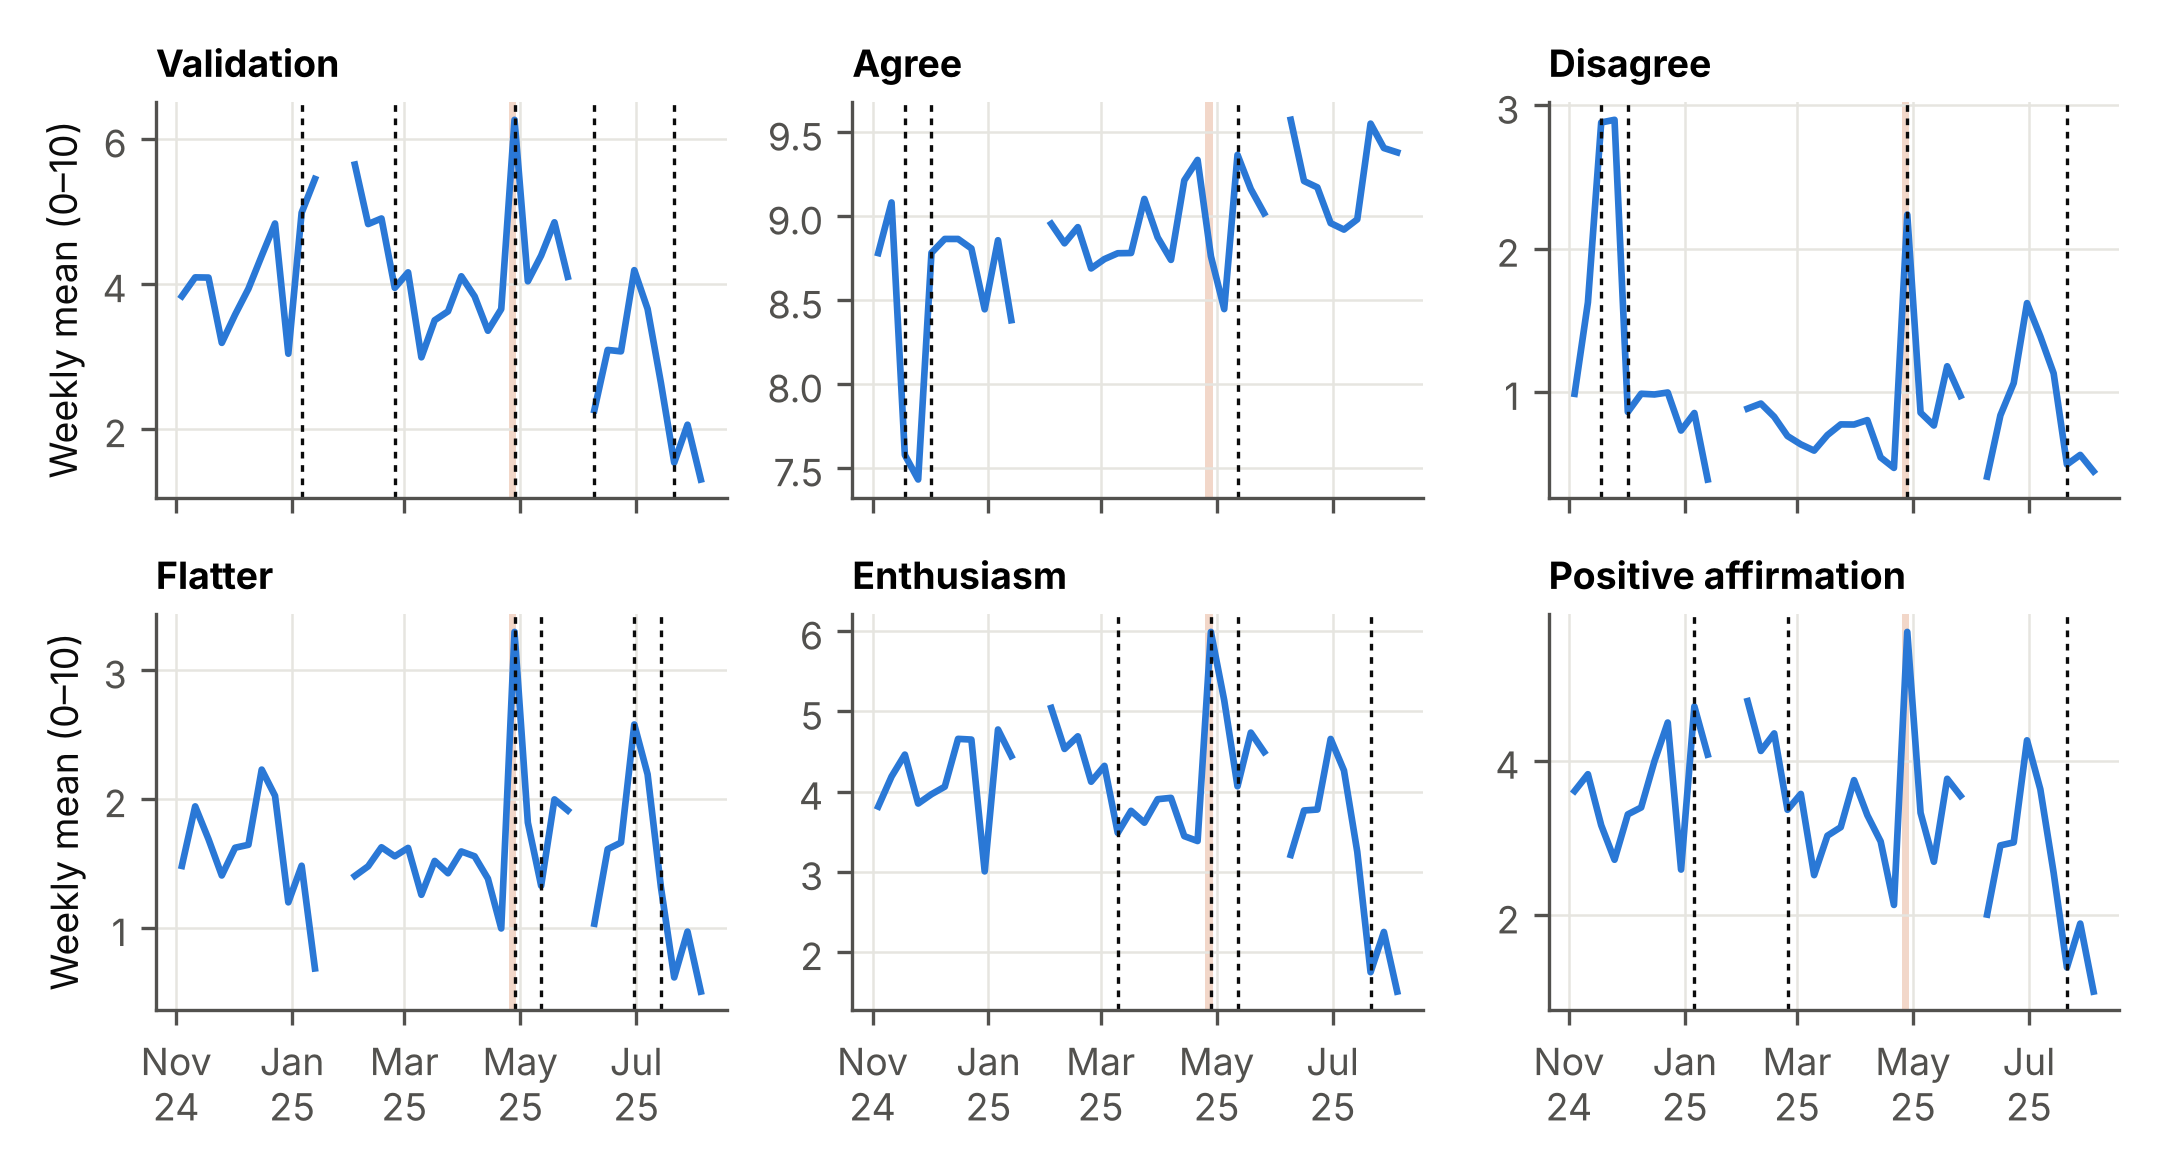
\includegraphics[width=\linewidth]{figures/appendix_all_traffic_six_criteria.png}
\caption{Weekly means of the six criteria, all traffic, supporting sample (12B), with PELT changepoints per criterion. The shaded band marks April 25--29.}
\label{fig:app-six}
\end{figure}

\FloatBarrier
\section{Serving history}\label{app:serving}
\begin{table}[h]
\caption{Model labels in a random sample of WildChat conversations, April 2023--July 2025, with the first and last day each label appears.}
\label{tab:app-serving}
\footnotesize
\setlength{\tabcolsep}{4pt}
\begin{adjustbox}{max width=\linewidth}
\begin{tabular}{@{}lrll@{}}
\toprule
Label & Turns & First & Last \\
\midrule
gpt-3.5-turbo-0301 & 1,650 & 2023-04-09 & 2023-06-28 \\
gpt-4-0314 & 230 & 2023-04-09 & 2023-06-24 \\
gpt-3.5-turbo-0613 & 2,030 & 2023-06-28 & 2024-02-16 \\
gpt-4-1106-preview & 693 & 2023-11-06 & 2024-03-14 \\
gpt-3.5-turbo-0125 & 774 & 2024-02-19 & 2024-08-06 \\
gpt-4-0125-preview & 602 & 2024-03-14 & 2024-05-06 \\
gpt-4-turbo-2024-04-09 & 181 & 2024-05-07 & 2024-07-07 \\
gpt-4o-2024-05-13 & 876 & 2024-05-13 & 2024-08-19 \\
gpt-4o-2024-08-06 & 4,114 & 2024-08-07 & 2024-11-20 \\
gpt-4o-mini-2024-07-18 & 2,762 & 2024-08-07 & 2025-04-14 \\
o1-mini-2024-09-12 & 111 & 2024-09-13 & 2025-01-03 \\
o1-preview-2024-09-12 & 147 & 2024-09-13 & 2025-01-04 \\
gpt-4o-2024-11-20 & 346 & 2024-12-01 & 2025-01-05 \\
gpt-4.1-mini-2025-04-14 & 2,362 & 2025-04-16 & 2025-07-31 \\
\bottomrule
\end{tabular}
\end{adjustbox}
\end{table}

\begin{table}[h]
\caption{Periods in which two labels were served at once (o1 labels excluded). The last ends on January 5, 2025.}
\label{tab:app-overlaps}
\footnotesize
\setlength{\tabcolsep}{4pt}
\begin{adjustbox}{max width=\linewidth}
\begin{tabular}{@{}llllr@{}}
\toprule
Label & Label & Start & End & Days \\
\midrule
gpt-3.5-turbo-0301 & gpt-4-0314 & 2023-04-09 & 2023-06-24 & 75 \\
gpt-3.5-turbo-0613 & gpt-4-1106-preview & 2023-11-06 & 2024-02-16 & 101 \\
gpt-3.5-turbo-0125 & gpt-4-1106-preview & 2024-02-19 & 2024-03-14 & 23 \\
gpt-3.5-turbo-0125 & gpt-4-0125-preview & 2024-03-14 & 2024-05-06 & 53 \\
gpt-3.5-turbo-0125 & gpt-4-turbo-2024-04-09 & 2024-05-07 & 2024-07-07 & 61 \\
gpt-4-turbo-2024-04-09 & gpt-4o-2024-05-13 & 2024-05-13 & 2024-07-07 & 54 \\
gpt-3.5-turbo-0125 & gpt-4o-2024-05-13 & 2024-05-13 & 2024-08-06 & 84 \\
gpt-4o-2024-05-13 & gpt-4o-2024-08-06 & 2024-08-07 & 2024-08-19 & 12 \\
gpt-4o-2024-05-13 & gpt-4o-mini-2024-07-18 & 2024-08-07 & 2024-08-19 & 12 \\
gpt-4o-2024-08-06 & gpt-4o-mini-2024-07-18 & 2024-08-07 & 2024-11-20 & 105 \\
gpt-4o-2024-11-20 & gpt-4o-mini-2024-07-18 & 2024-12-01 & 2025-01-05 & 34 \\
\bottomrule
\end{tabular}
\end{adjustbox}
\end{table}

